\chapter{Modulation Matrix}
\label{chapter_matrix}


\begin{center}
    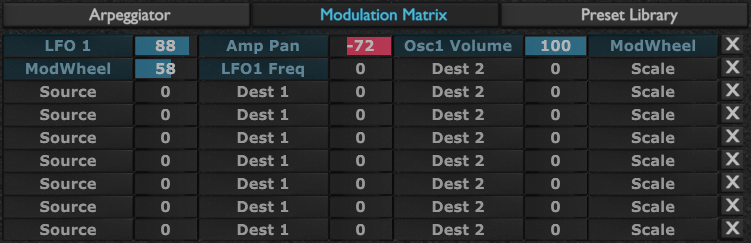
\includegraphics[width=0.9\textwidth]{graphics/modmatrix.png}
\end{center}

The modulation matrix is where the true power of Odin 2 lies. A large amount of parameters inside the synthesizer can be modulated by a large variety of modulators.

\section{Basic Operation}

It might look daunting at first with the amount of controls it has to offer, but in reality it is nine rows of the same controls:

\begin{center}
    
\includegraphics[width=0.9\textwidth]{graphics/modmatrix_row.png}
\end{center}

\audioparameter{Modulation Source}{0}{0}{
    Sets up a source for the modulation. The source chosen in this slot will be controlling the parameter set by "Destination 1" and "Destination 2" by the amounts set by "Destination 1 Amount" and "Destination 2 Amount".

    For a list of available modulation sources, see Section \ref{mod_sources}.
}

\audioparameter{Modulation Destination 1}{0}{0}{
    Sets up a destination for the modulation. The destination chosen in this slot will be controlled by the source set in "Modulation Source" by the amount set by "Destination 1 Amount".

    For a list of available modulation destinations, see Section \ref{mod_destinations}.
}

\audioparameter{Modulation Destination 2}{0}{0}{
    An independent second modulation destination with identical features to "Modulation Destination 1". Destinations 1 and 2 do not interfere with one another in any way.
}

\audioparameter{Destination 1 Amount}{0}{0}{
    Controls how much the Source modulates Destination 1. Can be positive or negative.
}

\audioparameter{Destination 2 Amount}{0}{0}{
    Controls how much the Source modulates Destination 2. Can be positive or negative.
}

You can use the X-Buttons to the right of each row to instantaneously clear the entire modulation row.

\section{Modulation Scaling}

An advanced feature of the modulation matrix in Odin 2 is the "Modulation Scale" option. You can scale the modulation that was set up with the parameters above by another modulation source. The value of the source chosen for scale now controls the modulation depth. This way you can essentially modulate the modulation itself. A common use case for this includes scaling with the Modwheel: The set up modulation now can be controlled by the keyboard player by moving the Modwheel up and down.

\vspace{10mm}
Consider the following graphic: On the left side, an LFO is set up to modulate a parameter. On the right side, the modulation is scaled by another, slower moving LFO:
\begin{center}
    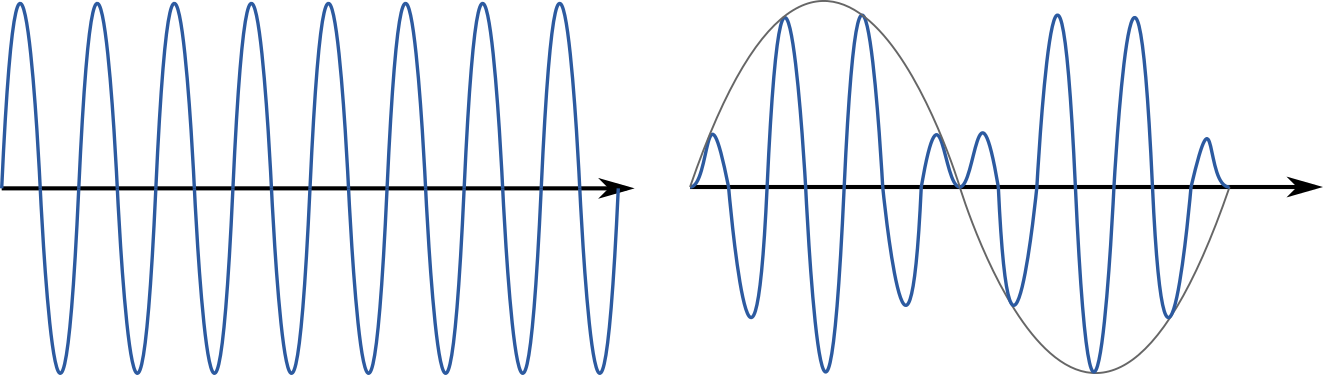
\includegraphics[width=\textwidth]{graphics/modulation_scale.png}
\end{center}
We can see how the actual modulation curve gets more complex instantaneously.

\audioparameter{Modulation Scale}{0}{0}{
    Select which modulation source is used to scale the modulations. Note that the scaling applies to Destination 1 and Destination 2 in the same way.

    For a list of available modulation sources, see Section \ref{mod_sources}.
}

\audioparameter{Scale Amount}{0}{0}{
    Determines the amount of scaling applied to the modulation. Using a scale amount of 100 is equivalent of multiplying the "Source" and "Scale" values together. For values between 0 and 100, linear interpolation logic applies between the raw modulation and and the multiplied values. For values below zero, the scaling source is inverted.
}

\section{Mono \& Poly Modulation}

Some of the modulation sources and destinations inside Odin 2 are polyphonic (i.e. exist once per voice), while others are monophonic (exist once per plugin instance). The following table summarizes the behavior when setting up poly/mono source and destination combos:

{\renewcommand{\arraystretch}{1.6}
\begin{tabular}{| L{0.2\textwidth} | L{0.35\textwidth} | L{0.35\textwidth} |}
    \hline
                                                              &
    \fat{Mono Destination}                                    &
    \fat{Poly Destination}                                      \\
    \hline
    \fat{Mono Source}                                         &
    single modulation source and destination                  &
    a single source modulates all destinations                  \\
    \hline
    \fat{Poly Source}                                         &
    only the most most recent voice modulates the destination &
    each voice is modulated independently                       \\
    \hline
\end{tabular}
}

\vspace{5mm}
A similar logic applies when dealing with poly/mono modulation scaling.

\vspace{5mm}
To see which modulations are poly or mono, refer to the tables in Section \ref{mod_sources} and Section \ref{mod_destinations}.

\section{Modulation Sources}
\label{mod_sources}
This list provides an overview over all modulation sources available in Odin 2:

Note that all unipolar sources operate in the range [0, 1], and all bipolar sources in the range [-1, 1].

\newcommand{\modsource}[4]{
    \fat{#1} &
    \IfEqCase{#2}{%
        {M}{Mono}%
            {P}{Poly}%
    }[\PackageError{audioparameter}{Undefined option to param: #2}{}]  &
    \IfEqCase{#3}{%
        {U}{Unipolar}%
            {B}{Bipolar}%
    }[\PackageError{audioparameter}{Undefined option to param: #3}{}] &
    #4 \\
    \hline
}

\vspace{5mm}
{\renewcommand{\arraystretch}{1.4}
    \begin{longtable}{| L{0.2\textwidth} | L{0.1\textwidth} | L{0.12\textwidth} |L{0.5\textwidth} |}
        \hline

        \fat{Source}     &
        \fat{Mono /Poly} &
        \fat{Polarity}   &
        \fat{Description}  \\
        \hline

        \modsource{Oscillator 1}{P}{B}{
            The output of the \hyperref[oscillators]{Oscillator} module that is currently in slot 1.
        }
        \modsource{Oscillator 2}{P}{B}{
            The output of the \hyperref[oscillators]{Oscillator} module that is currently in slot 2.
        }
        \modsource{Oscillator 3}{P}{B}{
            The output of the \hyperref[oscillators]{Oscillator} module that is currently in slot 3.
        }
        \modsource{Filter 1 Out}{P}{B}{
            The output of the \hyperref[filters]{Filter module} that is currently in slot 1. If no Filter is present, the bypassed signal is used.
        }
        \modsource{Filter 2 Out}{P}{B}{
            The output of the \hyperref[filters]{Filter module} that is currently in slot 2. If no Filter is present, the bypassed signal is used.
        }
        \modsource{Amp Envelope}{P}{U}{
            The \hyperref[ADSR]{Amplifier Envelope}.
        }
        \modsource{Filter Envelope}{P}{U}{
            The \hyperref[ADSR]{Filter Envelope}.
        }
        \modsource{Mod Envelope}{P}{U}{
            The \hyperref[ADSR]{Modulation Envelope}.
        }
        \modsource{Global Envelope}{M}{U}{
            The \hyperref[ADSR]{Global Envelope}.
        }
        \modsource{LFO 1}{P}{B}{
            The output of \hyperref[LFOs]{LFO 1}.
        }
        \modsource{LFO 2}{P}{B}{
            The output of \hyperref[LFOs]{LFO 2}.
        }
        \modsource{LFO 3}{P}{B}{
            The output of \hyperref[LFOs]{LFO 3}.
        }
        \modsource{Global LFO}{M}{B}{
            The output of the \hyperref[LFOs]{Global LFO}.
        }
        \modsource{X}{M}{U}{
            The X-coordinate of the \hyperref[xy]{XY-Pad}.
        }
        \modsource{Y}{M}{U}{
            The Y-coordinate of the \hyperref[xy]{XY-Pad}.
        }
        \modsource{Modwheel}{M}{U}{
            The position of the \hyperref[wheels]{Modwheel}.
        }
        \modsource{PitchBend}{M}{B}{
            The position of the \hyperref[wheels]{PitchBend wheel}.
        }
        \modsource{MIDI Note}{P}{U}{
            The index of the MIDI note-on event, scaled from 0 (note: 0, C-2) to 1 (note: 127, G8).
        }
        \modsource{MIDI Velocity}{P}{U}{
            The velocity of the MIDI note-on event, scaled from 0 (vel: 0) to 1 (vel: 127).
        }
        \modsource{MIDI Breath}{M}{U}{
            The MIDI Breath value (CC-2), often provided by dedicated breath controllers, scaled from 0 (CC-2: 0) to 1 (CC-2: 127).
        }
        \modsource{Channel Pressure}{M}{U}{
            Often referred to as "Mono Aftertouch". A pressure value applied to the keyboard after pressing a key, scaled from 0 (CP: 0) to 1 (CP: 127).
        }
        \modsource{Unison Index}{P}{B}{
            A unique value for each voice in a \hyperref[unison]{unison voice cluster}. The value is the one that is used to spread the voices over the stereo field.
        }
        \modsource{Arp Mod 1}{P}{B}{
            The upper row of modulation parameters from the \hyperref[arpeggiator]{Arpeggiator module}. This value is distributed to the voice that is triggered by that sequence step.
        }
        \modsource{Arp Mod 2}{P}{B}{
            The lower row of modulation parameters from the \hyperref[arpeggiator]{Arpeggiator module}. This value is distributed to the voice that is triggered by that sequence step.
        }
        \modsource{Sustain Pedal}{M}{U}{
            The pedal that is commonly used on (digital) pianos to avoid releasing keys.
        }
        \modsource{Soft Pedal}{M}{U}{
            The pedal that is commonly used on (digital) pianos to attenuate the volume of keys.
        }
        \modsource{Random}{P}{B}{
            A random value that is generated every time a new voice is triggered
        }
        \modsource{Constant}{M}{U}{
            A constant value of 1
        }
    \end{longtable}
}


\section{Modulation Destinations}
\label{mod_destinations}

This is an overview of all available modulation destinations in Odin 2. The column "Range" describes the amount of modulation that is applied if you use a "Constant" source and modulate by an amount of +100 or -100. Note that most destinations have internal logical limits for their modulation ranges. For example, the "Amplifier Pan" can not get out of the range [-1, 1].

\newcommand{\moddest}[5]{
    \fat{#1} &
    \IfEqCase{#2}{%
        {M}{\scriptsize{Mono}}%
            {P}{\scriptsize{Poly}}%
    }[\PackageError{audioparameter}{Undefined option to param: #2}{}]  &
    \footnotesize{#3} &
    \footnotesize{\fat{+100}: #4}

    \footnotesize{\fat{-100}: #5}\\
    \hline
}

\newcommand{\moddestcategory}[1]{
    \multicolumn{4}{|c|}{\fat{#1}} \\
    \hline
}

{\renewcommand{\arraystretch}{1.4}
    \begin{longtable}{| L{0.15\textwidth}| L{0.05\textwidth} | L{0.34\textwidth} | L{0.37\textwidth}|}
        \hline

        \fat{Destination}             &
        \scriptsize{\fat{Mono/ Poly}} &
        \fat{Description}             &
        \fat{Range}                     \\
        \hline

        \moddestcategory{Oscillator Common}

        \moddest{Osc Pitch Exp}{P}{
            Exponential modulation of the oscillator pitch}{
            Two octaves up}{
            Two octaves down}
        \moddest{Osc Pitch Lin}{P}{
            Linear modulation of the oscillator pitch}{
            Adds two times the current frequency}{
            Subtracts two times the current frequency, making the oscillator run backwards.}
        \moddest{Osc Volume}{P}{
            Modulates the volume of the oscillator
        }{
            If the volume is below -12dB, then modulation is up to 0dB. If the volume is above -12dB, then modulation is 12dB up from that point.
        }{
            Modulates to $-\infty$dB.
        }

        \moddestcategory{Analog Osc}
        \moddest{Pulse Width}{P}{
            Modulates the pulse width of the pulse wave. Unlike the control knob, this can be used to achieve a pulse-width of 0\% or 100\% (no sound) and beyond.
        }{
            Increase duty cycle by 100\%
        }{
            Decrease duty cycle by 100\%
        }
        \moddestcategory{Wavetable / Multi Osc}
        \moddest{Osc Position}{P}{
            Modulates the position used for interpolating between the four subtables.
        }{
            Move once through the entire table.
        }{
            Move once through the entire table backwards.
        }
        \moddestcategory{Multi Osc}

        \moddest{Osc Detune}{P}{
            Modulates the detuning of the sub-oscillators.
        }{
            Same as moving the control knob by a value of +1.
        }{
            Same as moving the control knob by a value of -1.
        }
        \moddest{Osc Spread}{P}{
            Modulates the spreading of the sub-oscillators across the wavetable.
        }{
            Same as moving the control knob by a value of +1.
        }{
            Same as moving the control knob by a value of -1.
        }
        \moddestcategory{Vector Osc}
        \moddest{Osc X}{P}{
            Modulate the X position of the vector pad.
        }{
            Move the handle the width of the pad to the right.
        }{
            Move the handle the width of the pad to the left.
        }
        \moddest{Osc Y}{P}{
            Modulate the Y position of the vector pad.
        }{
            Move the handle the height of the pad up.
        }{
            Move the handle the height of the pad down.
        }
        \moddestcategory{Chiptune Osc}
        \moddest{Osc Arp Speed}{P}{
            Modulates the speed of the arpeggiator in the chiptune osc exponentially.
        }{
            Increase the speed by a factor of 4.
        }{
            Decrease the speed by a factor of $1/4$.
        }
        \moddestcategory{FM and PhaseMod Oscs}
        \moddest{Osc FM amount}{P}{
            Modulates the amount of frequency modulation between carrier and modulator oscs.
        }{
            Same as moving the control knob by a value of +1.
        }{
            Same as moving the control knob by a value of -1.
        }
        \moddest{Osc PM amount}{P}{
            Modulates the amount of phase modulation between carrier and modulator oscs.
        }{
            Same as moving the control knob by a value of +1.
        }{
            Same as moving the control knob by a value of -1.
        }
        \moddest{Modulator Ratio}{P}{
            Modulates the ratio used for the modulator (see Section \ref{fm_osc}). Unlike the controls, this can be used to generate irrational fractions.
        }{
            Increases the current ratio by a factor of four.
        }{
            Decrease the current ratio by a factor of $1/4$.
        }
        \moddest{Carrier Ratio}{P}{
            Modulates the ratio used for the carrier (see Section \ref{fm_osc}). Unlike the controls, this can be used to generate irrational fractions.
        }{
            Increases the current ratio by a factor of four.
        }{
            Decrease the current ratio by a factor of $1/4$.
        }
        \moddestcategory{Noise Osc}
        \moddest{Osc LP Frequency}{P}{
            Modulates the frequency of the lowpass filter in the noise osc exponentially.
        }{
            Modulates the frequency 64 semitones up (factor 40.317).
        }{
            Modulates the frequency 64 semitones down (factor 0.0248).
        }
        \moddest{Osc HP Frequency}{P}{
            Modulates the frequency of the highpass filter in the noise osc exponentially.
        }{
            Modulates the frequency 64 semitones up (factor 40.317).
        }{
            Modulates the frequency 64 semitones down (factor 0.0248).
        }
        \moddestcategory{Filter Common}
        \moddest{Filter Frequency}{P}{
            Modulates the filter frequency exponentially.
        }{
            Modulates the frequency 64 semitones up (factor 40.317).
        }{
            Modulates the frequency 64 semitones down (factor 0.0248).
        }
        \moddest{Filter Resonance}{P}{
            Modulates the resonance of the filter.
        }{
            Same as moving the control knob by a value of +1.
        }{
            Same as moving the control knob by a value of -1.
        }
        \moddest{Filter Gain}{P}{
            Modulates the volume of the filter.
        }{
            If the current gain is below -12dB, then modulation is up to 0dB. If the gain is above -12dB, then modulation is 12dB up from that point.
        }{
            Modulates to $-\infty$dB.
        }
        \moddest{Filter Env Amount}{P}{
            Modulates how much envelope is applied to the filter.
        }{
            Same as moving the control knob by a value of +1.
        }{
            Same as moving the control knob by a value of -1.
        }
        \moddest{Filter Vel Amount}{P}{
            Modulates the velocity sensitivity of the filter.
        }{
            Same as moving the control knob by a value of +1.
        }{
            Same as moving the control knob by a value of -1.
        }
        \moddest{Filter Kbd Amount}{P}{
            Modulates the keyboard sensitivity of the filter.
        }{
            Same as moving the control knob by a value of +1.
        }{
            Same as moving the control knob by a value of -1.
        }
        \moddest{Filter Saturation}{P}{
            Modulates the saturation of the filter.
        }{
            Same as moving the control knob by a value of +1.
        }{
            Same as moving the control knob by a value of -1.
        }
        \moddestcategory{SEM-12 Filter}
        \moddest{Filter SEM Transition}{P}{
            Modulates the filter characteristic transition from lowpass over notch to highpass.
        }{
            Same as moving the control knob by a value of +1.
        }{
            Same as moving the control knob by a value of -1.
        }
        \moddestcategory{Formant Filter}
        \moddest{Filter Formant Transition}{P}{
            Modulates the transition from the left vowel to the right.
        }{
            Same as moving the control knob by a value of +1.
        }{
            Same as moving the control knob by a value of -1.
        }
        \moddestcategory{Amplifier}
        \moddest{Amplifier Gain}{P}{
            Modulates the gain in the Amplifier module.
        }{
            If the current gain is below -12dB, then modulation is up to 0dB. If the gain is above -12dB, then modulation is 12dB up from that point.
        }{
            Modulates to $-\infty$dB.
        }
        \moddest{Amplifier Pan}{P}{
            Modulates the position of the sound in the stereo field.
        }{
            Same as moving the control knob by a value of +1.
        }{
            Same as moving the control knob by a value of -1.
        }
        \moddestcategory{Distortion}
        \moddest{Distortion Boost}{P}{
            Modulates the input boost of the distortion module.
        }{
            Same as moving the control knob by a value of +1.
        }{
            Same as moving the control knob by a value of -1.
        }
        \moddest{Distortion DryWet}{P}{
            Modulates the relation of unprocessed and processed signal in the Distortion module.
        }{
            Same as moving the control knob by a value of +1.
        }{
            Same as moving the control knob by a value of -1.
        }
        \moddestcategory{ADSR Envelopes}
        \moddest{Env Attack}{P}{
            Modulates the attack time of the Envelope exponentially and linearly. This parameter is Mono for the Global Env.
        }{
            Scales the current time by a factor of 8 and then adds 0.3 seconds.
        }{
            Scales the current time by a factor of $1/8$ and then subtracts 0.3 seconds.
        }
        \moddest{Env Decay}{P}{
            Modulates the decay time of the Envelope exponentially and linearly. This parameter is Mono for the Global Env.
        }{
            Scales the current time by a factor of 8 and then adds 0.3 seconds.
        }{
            Scales the current time by a factor of $1/8$ and then subtracts 0.3 seconds.
        }
        \moddest{Env Sustain}{P}{
            Modulates the sustain value of the Envelope.
        }{
            Same as moving the control slider +1.
        }{
            Same as moving the control slider -1.
        }
        \moddest{Env Release}{P}{
            Modulates the release time of the Envelope exponentially and linearly. This parameter is Mono for the Global Env.
        }{
            Scales the current time by a factor of 8 and then adds 0.3 seconds.
        }{
            Scales the current time by a factor of $1/8$ and then subtracts 0.3 seconds.
        }
        \moddestcategory{LFOs}
        \moddest{LFO Freq}{P}{
            Modulates the frequency of the LFO exponentially. This parameter is Mono for the Global LFO.
        }{
            Increases current frequency by 4 octaves (factor 16).
        }{
            Decreases current frequency by 4 octaves (factor 0.0625).
        }
        \moddestcategory{Delay}
        \moddest{Delay Time}{M}{
            Modulates the delay time exponentially.
        }{
            Increases the current time by a factor of 3.
        }{
            Decreases the current time by a factor of $1/3$.
        }
        \moddest{Delay Feedback}{M}{
            Modulates the feedback of the delay line.
        }{
            Same as moving the control knob by a value of +1.
        }{
            Same as moving the control knob by a value of -1.
        }
        \moddest{Delay HP Freq}{M}{
            Modulates the frequency of the highpass filter in the Delay module exponentially.
        }{
            Modulates the frequency 64 semitones up (factor 40.317).
        }{
            Modulates the frequency 64 semitones down (factor 0.0248).
        }
        \moddest{Delay Dry}{M}{
            Modulates the output of unprocessed signal from the Delay module.
        }{
            Same as moving the control knob by a value of +1.
        }{
            Same as moving the control knob by a value of -1.
        }
        \moddest{Delay Wet}{M}{
            Modulates the output of processed signal from the Delay module.
        }{
            Same as moving the control knob by a value of +1.
        }{
            Same as moving the control knob by a value of -1.
        }
        \moddestcategory{Phaser}
        \moddest{Phaser Rate}{M}{
            Modulates the speed of the internal LFO exponentially.
        }{
            Increases the speed by a factor of 4.
        }{
            Decreases the speed by a factor of $1/4$.
        }
        \moddest{Phaser Amount}{M}{
            Modulates the depth of frequency modulation by the LFO in the Phaser.
        }{
            Same as moving the control knob by a value of +1.
        }{
            Same as moving the control knob by a value of -1.
        }
        \moddest{Phaser Freq}{M}{
            Modulates the base frequency of the internal allpass filters linearly.
        }{
            Moves the frequency up 2000Hz.
        }{
            Moves the frequency down 2000Hz.
        }
        \moddest{Phaser Feedback}{M}{
            Modulates the internal feedback of the Phaser module.
        }{
            Same as moving the control knob by a value of +1.
        }{
            Same as moving the control knob by a value of -1.
        }
        \moddest{Phaser Drywet}{M}{
            Modulates the ratio of processed and unprocessed signals output by the Phaser module.
        }{
            Same as moving the control knob by a value of +1.
        }{
            Same as moving the control knob by a value of -1.
        }
        \moddestcategory{Chorus}
        \moddest{Chorus Rate}{M}{
            Modulates the speed of the internal LFO exponentially.
        }{
            Increases the speed by a factor of 4.
        }{
            Decreases the speed by a factor of $1/4$.
        }
        \moddest{Chorus Amount}{M}{
            Modulates the depth of frequency modulation by the LFO in the Chorus.
        }{
            Same as moving the control knob by a value of +1.
        }{
            Same as moving the control knob by a value of -1.
        }
        \moddest{Chorus Feedback}{M}{
            Modulates the feedback of the internal delay line.
        }{
            Same as moving the control knob by a value of +1.
        }{
            Same as moving the control knob by a value of -1.
        }
        \moddest{Chorus Drywet}{M}{
            Modulates the ratio of processed and unprocessed signals output by the Chorus module.
        }{
            Same as moving the control knob by a value of +1.
        }{
            Same as moving the control knob by a value of -1.
        }
        \moddestcategory{Flanger}
        \moddest{Flanger Rate}{M}{
            Modulates the speed of the internal LFO exponentially.
        }{
            Increases the speed by a factor of 4.
        }{
            Decreases the speed by a factor of $1/4$.
        }
        \moddest{Flanger Amount}{M}{
            Modulates the depth of frequency modulation by the LFO in the Flanger.
        }{
            Same as moving the control knob by a value of +1.
        }{
            Same as moving the control knob by a value of -1.
        }
        \moddest{Flanger Feedback}{M}{
            Modulates the feedback of the internal delay line.
        }{
            Same as moving the control knob by a value of +1.
        }{
            Same as moving the control knob by a value of -1.
        }
        \moddest{Flanger Drywet}{M}{
            Modulates the ratio of processed and unprocessed signals output by the Flanger module.
        }{
            Same as moving the control knob by a value of +1.
        }{
            Same as moving the control knob by a value of -1.
        }
        \moddestcategory{Arpeggiator}
        \moddest{Arp Speed}{M}{
            Modulates the speed of the Arpeggiator module exponentially
        }{
            Doubles the speed.
        }{
            Halves the speed.
        }
        \moddest{Arp Gate}{M}{
            Modulates the gate time in the Arpeggiator module.
        }{
            Adds 100\% gate time.
        }{
            Subtracts 100\% gate time.
        }
        \moddestcategory{XY-Pad}
        \moddest{XY-Pad X}{M}{
            Modulates X coordinate of the XY-Pad in the synth (see Section \ref{xy}).
        }{
            Like moving the handle once across the pad to the right.
        }{
            Like moving the handle once across the pad to the left.
        }
        \moddest{XY-Pad Y}{M}{
            Modulates Y coordinate of the XY-Pad in the synth (see Section \ref{xy}).
        }{
            Like moving the handle once across the pad upwards.
        }{
            Like moving the handle once across the pad downwards.
        }
        \moddestcategory{Global}
        \moddest{Glide}{M}{
            Modulates the Glide parameter in the synth (see Section \ref{glide}).
        }{
            Same as moving the control knob by a value of +1.
        }{
            Same as moving the control knob by a value of -1.
        }
        \moddest{Master}{M}{
            Modulates the master gain of the synthesizer.
        }{
            If the current master gain is below -12dB, then modulation is up to 0dB. If the master gain is above -12dB, then modulation is 12dB up from that point.
        }{
            Modulates to $-\infty$dB.
        }
    \end{longtable}
}
